\documentclass[a4paper,12pt]{article}
\usepackage[latin1]{inputenc}
\usepackage[spanish]{babel}
\usepackage{bm}
\usepackage{graphicx}
\usepackage{amsmath}
\setlength{\textheight}{235mm}
\setlength{\textwidth}{168mm}
\setlength{\oddsidemargin}{0pt}
\pagestyle{empty}
\begin{document}
\mbox{}\vspace*{-45mm}

{\centering
{\small\sc Escuela T�cnica Superior de Ingenieros de Caminos, Canales y
Puertos (Madrid)}\\*[4mm]
{\Large\bf M�todo de los Elementos Finitos (Curso 17-18)}\\*[4mm]
Ejercicio 2: Ecuaci�n de difusi�n \\*[4mm]
}

\vspace{3mm}

%%%%%
\noindent
La figura muestra la secci�n transversal de un r�o canalizado, en una zona en la
que se ha contru�do un tunel provisional de $5$ m de longitud y secci�n cuadrada
de $1$ m de lado. El extremo derecho del tunel est� a la presi�n atomosf�rica.
El terreno tiene un coeficiente de permeabilidad $k=10^{-3}$ m/s y est� 
confinado por pantallas impermeables y terreno igualmente impermeable.

Para analizar las filtraciones que se producen se realizar� un modelo plano
de elementos finitos que represente dicha secci�n transversal.
La discretizaci�n a efectuar corresponde a elementos cuadrados de cuatro
nodos de lado $0.2$ m.

\begin{center}
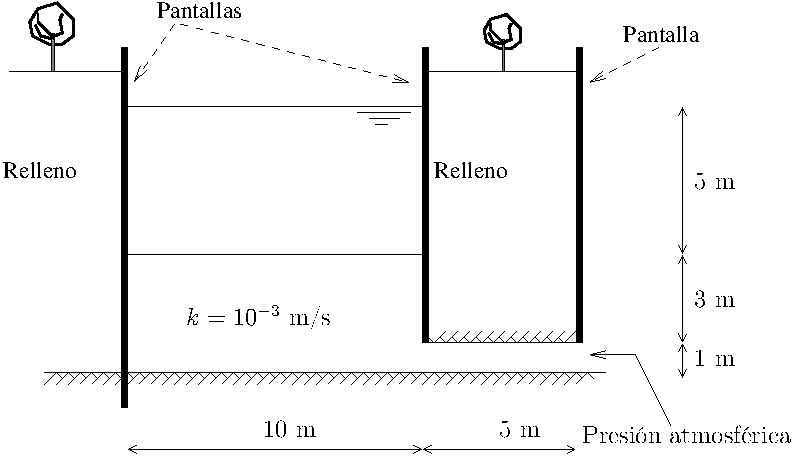
\includegraphics[width=0.75\textwidth]{practi2}
\end{center}

\end{document}
